In these laboratory assignement the objective is to use an AC/DC converter to obtain a DC signal as an output. The DC signal must be a value of 12V from an AC signal with an amplitude of 230V and a frequency of 50Hz. The envelope detector and voltage regulator circuits were chosen by us as shown in Figure... 


 \FloatBarrier 
 \begin{center}
\begin{figure}
  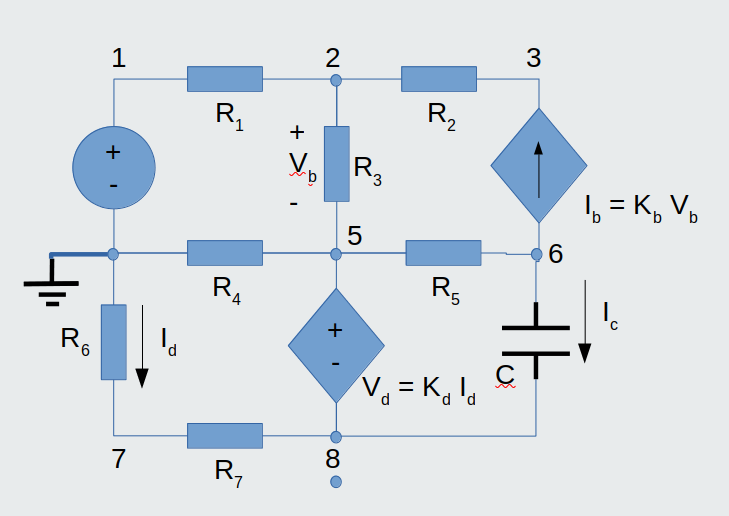
\includegraphics[width=\linewidth]{circuit.JPG}
  \caption{The circuit used in this laboratory}
  \label{fig:circuit}
\end{figure}
\end{center}
\FloatBarrier


% colocar figura do circuito com a configuração utilizada.
